\documentclass[11pt,twocolumn]{article}
\usepackage[a4paper,margin=0.67in,columnsep=0.24in]{geometry}
\usepackage[T1]{fontenc}
\usepackage{mathptmx}
\usepackage{microtype,graphicx,booktabs,amsmath,array,xcolor}
\usepackage[numbers,sort&compress]{natbib}
\usepackage{titlesec,enumitem,caption,fancyhdr}
\usepackage[colorlinks=true,urlcolor=blue!50!black,citecolor=blue!50!black,linkcolor=blue!50!black]{hyperref}
\usepackage{xurl}
\hypersetup{pdftitle={Keep Learning or Start Over? Plasticity-Preserving Updates for Bearing Vibration Forecasting},pdfauthor={Elissa Ephrem; Galia Akkl; Karim Bteish},pdfsubject={Introduction to Machine Learning project proposal, AUB, Fall 2026}}
\titleformat{\section}{\normalsize\bfseries\color{blue!35!black}}{\thesection.}{0.45em}{}
\titlespacing*{\section}{0pt}{6pt}{3pt}
\setlength{\parindent}{0pt}\setlength{\parskip}{3pt}
\raggedbottom
\clubpenalty=10000\widowpenalty=10000
\setlength{\textfloatsep}{8pt}\setlength{\intextsep}{7pt}
\captionsetup{font=small,labelfont=bf,skip=4pt}
\setlist{leftmargin=*,nosep}
\pagestyle{fancy}\fancyhf{}
\fancyfoot[L]{\footnotesize Introduction to Machine Learning \textbar\ AUB \textbar\ Fall 2026}
\fancyfoot[R]{\footnotesize\thepage}
\renewcommand{\headrulewidth}{0pt}\renewcommand{\footrulewidth}{0.3pt}
\setlength{\headheight}{12pt}
\newcommand{\rms}{\operatorname{RMS}}
\begin{document}
\twocolumn[{
\begin{center}
{\LARGE\bfseries Keep Learning or Start Over?}\par\vspace{3pt}
{\large Plasticity-Preserving Updates for Bearing Vibration Forecasting}\par\vspace{5pt}
{\small\begin{tabular}{ccc}
Elissa Ephrem & Galia Akl & Karim Bteish \\
\href{mailto:eee19@mail.aub.edu}{\texttt{eee19@mail.aub.edu}} &
\href{mailto:gra16@mail.aub.edu}{\texttt{gra16@mail.aub.edu}} &
\href{mailto:krb05@mail.aub.edu}{\texttt{krb05@mail.aub.edu}}
\end{tabular}}\par
{\small Project proposal \textbar\ 20 October 2026 }\par
\end{center}\vspace{-2pt}
}]

\section{Problem and motivation}
As a bearing degrades, a vibration forecaster may need updating. However, continued training can reduce a neural network's ability to learn new patterns, a phenomenon called \emph{loss of plasticity}~\citep{dohare2024}. We ask: \textbf{do simple plasticity-preserving updates improve one-hour-ahead vibration forecasting relative to ordinary continual training and periodic retraining, at comparable computational cost?} A secondary question is whether internal diagnostics predict \emph{when an intervention helps}, rather than merely tracking current error.

We will predict $y_t=\log_{10}[\rms(t+1\,\mathrm{h})/(1\,g)]$ from current and past vibration features. This is a regression task, not a remaining-useful-life (RUL) estimator or failure alarm. Our measurable objective is positive forecasting skill, $1-\mathrm{MAE}_{m}/\mathrm{MAE}_{b}>0$, against both ordinary updating and a validation-selected periodic-retraining baseline on the evaluation run. We also require comparison with persistence and inspection of late-life errors; success is not assumed.

\section{Impact}
The practical decision is whether a monitoring model should retain its weights, refresh a small part of them, or restart. A useful result identifies an accuracy--computation trade-off that maintenance analysts can examine before adopting costly adaptation. A negative result is also informative: resets may harm useful representations, or improved trainability may not improve forecasting. Underprediction during degradation is especially concerning, so we report directional and late-life errors. One laboratory rig and few failures cannot establish industrial safety or generalization. No maintenance decisions will be automated.

\section{Related work and positioning}
\textbf{Warm starts.} \citet{ash2020} found that warm-starting can generalize worse than fresh initialization despite similar training losses, and introduced shrink-and-perturb. We reuse that lightweight intervention, but evaluate chronological vibration forecasting rather than assume its gains transfer.

\textbf{Sustained learning.} \citet{dohare2024} demonstrated plasticity loss in continual image-learning and reinforcement-learning settings; continual backpropagation recycles low-utility units. Their evidence motivates equal-budget trainability comparisons. We do not assume their phenomenon must appear in every bearing history.

\textbf{Selective resets.} \citet{sokar2023} linked increasing neuron dormancy to reduced expressivity in reinforcement learning and proposed ReDo. We test a documented ReDo-style intervention in regression, keeping architecture and data access fixed.

\textbf{Interpreting diagnostics.} \citet{lyle2023} connected plasticity loss to loss-landscape curvature, including cases without saturated units. Thus, neuron inactivity alone will not be treated as proof of the mechanism. In a recent preprint, \citet{wang2026} showed that rank-based diagnostics can fail to predict trainability and proposed optimization readiness. We distinguish trainability from the subsequent forecasting benefit of a specific intervention; implementing their full diagnostic is outside the core scope.

\textbf{Closest bearing application.} \citet{yang2026} combine BiGRU--Informer fusion with utility-based selective reinitialization for RUL prediction. Their XJTU-SY ablations report lower errors with the plasticity mechanism; supplementary FEMTO-ST experiments extend evaluation. They use successive groups of bearing histories. We found no explicit matched-budget periodic-retraining comparison or evaluation of diagnostics as predictors of future intervention benefit. Our contribution is that controlled comparison for a small chronological RMS forecaster, building on established bearing-plasticity work. We claim neither a new reset algorithm nor the first bearing application.

\begin{figure*}[t]
\centering
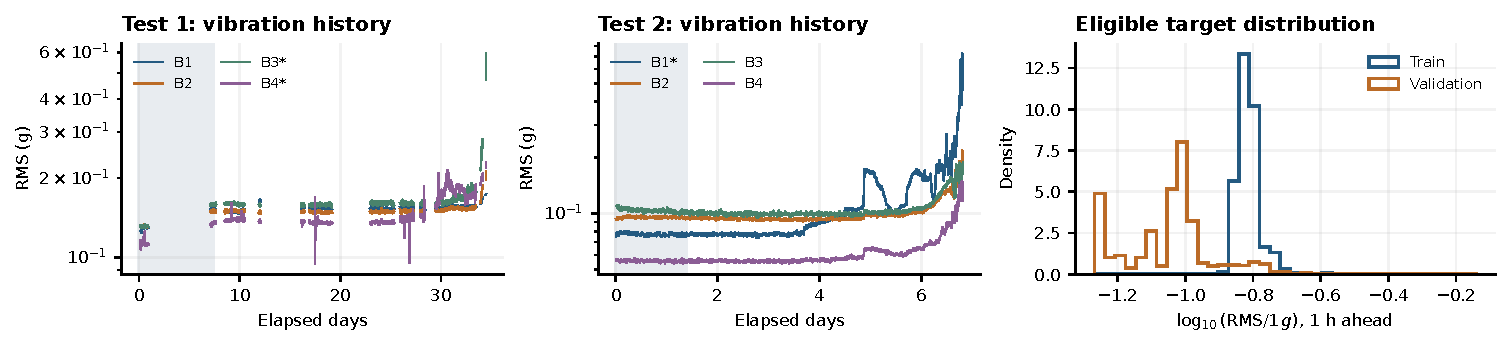
\includegraphics[width=\textwidth]{figures/data_overview.pdf}
\caption{Recomputed exploration of Tests 1--2. Left: unsmoothed RMS histories; * marks a documented failed bearing, gray marks the first 200 calibration observations, and lines break at irregular intervals. Right: target distributions after filtering. These are vibration forecasts, not failure-class labels. Source: supplied IMS-derived feature tables~\citep{ims,features}; figure generated by the accompanying baseline script.}
\label{fig:data}
\end{figure*}

\section{Data and preliminary exploration}
\textbf{Source and access.} The IMS Bearing Data Set was collected by the University of Cincinnati's Center for Intelligent Maintenance Systems with Rexnord and distributed through NASA~\citep{ims,qiu2006}. The official entry is \url{https://data.nasa.gov/dataset/ims-bearings}. It labels the license \texttt{other-license-specified} and links U.S. government-work guidance; we preserve source acknowledgements and do not infer that third-party code licensing licenses the raw data.

Our starting point is six processed CSVs from the public \texttt{nasa-bearing-anomaly} repository~\citep{features}. All supplied files were byte-matched to commit \texttt{f8a40f9} on 20 October 2026; the repository's code is MIT-licensed. This verifies the feature-table source, not the original extraction. Week 1 includes checking representative early/late raw recordings and acquisition metadata before relying on spectral interpretations.

The rig records four bearings at 2,000 rpm under a 6,000-lb radial load, with 20,480-sample accelerometer snapshots at nominal 20 kHz~\citep{qiu2006,features}. Tests 1--3 provide 2,156, 984 and 6,324 acquisition rows; Test 1 has two channels per bearing and the others one. We use channel 1 throughout. There are 12 bearing histories but only three runs and four documented failures; co-mounted bearings and adjacent rows are dependent.



\textbf{Inputs and preprocessing.} Twenty continuous features comprise RMS/std/peak ($g$), four shape ratios, PSD mean/std and six defect-band sums (upstream PSD units, $g^2/\mathrm{Hz}$), three shape statistics, spectral entropy and a high-frequency ratio (dimensionless). Six-observation trailing means give 40 inputs. Positive scale features are log-transformed; signed shape statistics use a signed logarithm. Each bearing's first 200 observations calibrate the mean/std; an $\operatorname{asinh}$ transform compresses extremes. Calibration observations are excluded from fitting and scoring. Rolling windows restart at gaps. We retain six-step pairs only when intervening intervals are 9--11 min and elapsed horizon is $60\pm1$ min, with a complete trailing history.

\begin{table}[t]
\centering\small\setlength{\tabcolsep}{3pt}
\caption{Recomputed development-data audit. Forecast counts include all four bearings; zero missing entries were found.}
\begin{tabular}{@{}lrr@{}}\toprule
Quantity & Test 1 & Test 2 \\\midrule
Original / live snapshots & 2,156 / 2,156 & 984 / 982 \\
Eligible forecast pairs & 6,428 & 3,104 \\
Gaps $>15$ min & 24 & 0 \\
Target mean / SD & $-0.813$ / 0.035 & $-1.046$ / 0.138 \\
Late failed-bearing pairs & 558 & 99 \\\bottomrule
\end{tabular}\label{tab:data}
\end{table}

Only the trailing acquisitions where \emph{all four} channels fall below 20\% of their calibration-median RMS are removed (two in Test 2). Test 1 has a 6.18-day gap. Snapshot noise, few failures, one operating condition and shared-shaft vibration limit conclusions; a bearing without a documented failure is not an independently certified healthy control. Figure~\ref{fig:data} shows concentrated targets with a degradation tail. No interpolation or future-derived failure label is used as an input.

\section{Models and preliminary baseline}
\textbf{Simple baselines.} Last-value and moving-average persistence encode short-horizon continuity. Ridge regression~\citep{ridge} predicts the residual from the trailing mean of log-RMS, testing whether the 40 features add linear predictive information. Training uses Test 1; seven ridge penalties $10^0$--$10^6$ were compared on Test 2, selecting $\lambda=100$ for the unnormalized squared-error objective. Table~\ref{tab:base} reports the reproduced baseline results. Late means target time within the final 10\% of elapsed live-run time, on documented failed bearings only.

\begin{table}[t]
\centering\small\setlength{\tabcolsep}{3pt}
\caption{Executed baselines: log-RMS MAE (lower is better). Train error is in-sample; validation error is out of run.}
\begin{tabular}{@{}lrrr@{}}\toprule
Model & Train & Validation & Val. late \\\midrule
Last-value persistence & 0.00379 & 0.01128 & 0.06936 \\
Moving-average persistence & 0.00336 & 0.01124 & 0.07699 \\
Ridge residual & 0.00338 & 0.01115 & 0.07594 \\
Static MLP (seed 42) & 0.00336 & 0.01110 & 0.07616 \\\bottomrule
\end{tabular}\label{tab:base}
\end{table}

Ridge and the static MLP offer small overall validation-MAE gains; last-value persistence is better late in life. The MLP has slightly worse validation RMSE than ridge (0.02585 versus 0.02567). One selected seed does not establish superiority or plasticity loss.

\textbf{One neural architecture.} We implemented a 40--64--64--1 ReLU MLP (6,849 parameters) in NumPy~\citep{numpy}, including backpropagation and Adam~\citep{adam}; all 49 parameters of a small version passed a finite-difference gradient check. It predicts the same residual, scaled by its training-only standard deviation, using MSE, batch size 64 and learning rate $10^{-3}$. Test-2 MAE selected epoch 1; patience 25 stopped training at epoch 26. Further training lowered training error but raised validation error. These scores were reproduced on a teammate's laptop. The planned adaptive methods start from independent source-model copies for each bearing.

\textbf{Four update strategies.} (i) ordinary continual updates; (ii) periodic full reinitialization followed by retraining; (iii) shrink-and-perturb, $\theta\leftarrow\alpha\theta+\sigma\theta_0$~\citep{ash2020}; and (iv) ReDo-style resets of low relative-activation units~\citep{sokar2023}, reinitializing incoming weights, zeroing outgoing weights and clearing affected optimizer state. Strategy (ii) continues updating between restarts. It tests whether preserving old weights is useful; (iii)--(iv) test gentler alternatives.

\textbf{Causal updates and cost.} At six-hour update times, each model uses at most the latest 200 eligible examples whose targets have already arrived; its buffer is cleared at acquisition gaps. All adaptive strategies receive the same examples, batch size and step allowance (25 or 100 steps/update). Test 2 selects restart/intervention frequency from 24 or 48 h and a small strength grid, with at most eight configurations per strategy. Initialization, optimizer resets, data access and timing will be logged. An additional retraining run with four times the step allowance checks whether strict budget limits unfairly handicap restarts; it is compared on an accuracy--cost curve, not called equal-cost.

\section{Evaluation and diagnostic study}
\textbf{Split and reporting.} Test 1 trains the source models; Test 2 selects settings; Test 3 is evaluated after settings are frozen. Test 3 has been inspected descriptively, so it is not a pristine blind dataset; no Test-3 model scores are used here. Online Test-3 updates are allowed only after labels mature, with predictions saved first. We report macro-average per-bearing MAE, pooled MAE/RMSE, late-life MAE and mean underprediction $\max(y-\hat y,0)$, plus runtime, update count and reset count. Log-space errors will not be mislabeled as percentage errors.

Five paired seeds share initial weights and minibatch schedules where applicable. We will report each bearing and seed, paired error differences, and descriptive 95\% moving-block bootstrap intervals (24-h blocks, 48-h sensitivity) within each run; co-mounted bearings stay grouped. These intervals describe this record, not population-level reliability. All methods use identical preprocessing; published RUL/classification scores are not numerical benchmarks for this target. Ablations include a 400-example buffer, 12-h updates and removing the range-compression transform, varied one at a time.

\textbf{Secondary: predict intervention benefit.} Every 24 h, copies of an ordinary continual checkpoint branch into continue, selected intervention, and fresh retraining. Each receives the same matured buffer and update budget; the branches remain frozen while forecasting the next non-overlapping 24 h. We define $\Delta=\mathrm{MAE}_{\rm continue}-\mathrm{MAE}_{\rm intervention}$. Before branching, we record dormant fraction and normalized effective rank~\citep{roy2007}; we compare their ability to rank $\Delta$ with recent matured-label error and cumulative update count. Directions/thresholds are selected on Test 2, then evaluated on Test 3 using Spearman correlation and AUROC for $\Delta>0$ (undefined if only one outcome class occurs). Future scores never trigger a past action.

\textbf{Interpretation and fallback.} A controlled probe on copies, with matched output initialization, reset optimizer state, identical targets and budget, will compare warm/fresh learning curves. A small synthetic changing-target stream checks that the implementation can expose plasticity loss. Neither random-target fit nor rank alone proves useful adaptation or causality. If the real stream shows little loss, that negative result will be reported without repeated data recycling. The core forecasting comparison remains the deliverable; a learned intervention policy and second dataset are optional.

\section{Resources and code}
The laptop-first implementation uses Python, NumPy, pandas~\citep{pandas} and Matplotlib~\citep{matplotlib}. The accompanying code includes the loader, simple and neural baselines, checksums, compact results and setup README; running it regenerates per-example predictions. The reproduced static MLP run took 1.36 s excluding plotting; this does not predict the full grid's cost. We initially budget 10--30 CPU-hours and will profile before expanding. AUB HPC and GPU computation are not required for the core scope. All members will commit regularly, review generated code and disclose AI assistance. Continual-update and plasticity experiments remain planned.

\textbf{Code repository:}
\url{https://github.com/karimbteish/plasticity-bearing-forecasting}

\section{Timeline and responsibilities}
\small
Elissa Ephrem leads data/provenance; Galia Akl leads models/updates; Karim Bteish leads evaluation/diagnostics. All three contribute code and writing.

\begin{tabular}{@{}p{.16\columnwidth}p{.78\columnwidth}@{}}\toprule
Week & Milestone and owner \\\midrule
Oct 19 & Proposal Oct 20; audit, baseline, repository (all). \\
Oct 26 & Raw-data spot-check; timestamp/unit audit (Elissa); static MLP seed and learning-rate checks (Galia). \\
Nov 2 & Causal stream, retraining and two interventions (Galia); paired logging and cost profiling (Karim). \\
Nov 9 & Test-2 tuning; freeze primary protocol (Galia/Karim); checkpoint-branch pilot and data review (Elissa/Karim). \\
Nov 16 & Progress report Nov 17 (all); five-seed development results and selected ablations (Galia/Karim). \\
Nov 23 & Frozen Test-3 evaluation; uncertainty and diagnostic analysis (Elissa/Karim); finalize scope (all). \\
Nov 30 & Figures, poster and rehearsal; poster session Dec 4 (all). \\
Dec 7 & Final report, limitations and reproducibility; submit Dec 10 (all). \\\bottomrule
\end{tabular}
\normalsize

\clearpage
\bibliographystyle{unsrtnat}
\setlength{\bibsep}{4pt}
\small
\bibliography{refs}
\end{document}
